\documentclass[11pt,a4paper]{article}
\usepackage[margin=2.5cm]{geometry}
\usepackage{amsmath,amssymb,amsthm}
\usepackage{graphicx}
\usepackage{enumitem}
\usepackage{tikz}
\usetikzlibrary{decorations.pathmorphing,patterns}
\usepackage{fancyhdr}
\usepackage{multicol}
\usepackage{xcolor}
\usepackage{tcolorbox}
\tcbuselibrary{skins,breakable}
\usepackage{hyperref}
\usepackage{float}
\usepackage{wrapfig}

% Define company colors
\definecolor{yolyblue}{RGB}{41, 128, 185}
\definecolor{yolylightblue}{RGB}{174, 214, 241}
\definecolor{yolygray}{RGB}{236, 240, 241}
\definecolor{yolydarkblue}{RGB}{21, 67, 96}
\definecolor{cosmicpurple}{RGB}{123, 44, 191}
\definecolor{cosmicgold}{RGB}{241, 196, 15}

% Hyperlink setup
\hypersetup{
    colorlinks=true,
    linkcolor=yolyblue,
    urlcolor=yolyblue,
    citecolor=yolyblue
}

% Header and footer
\pagestyle{fancy}
\fancyhf{}
\fancyhead[L]{\small\textit{CMB \& Early Universe}}
\fancyhead[R]{\small\textbf{Yolymatics Tutorials}}
\fancyfoot[C]{\small Page \thepage}
\fancyfoot[R]{\small\textcolor{yolyblue}{\href{http://www.yolymaticstutorials.com}{www.yolymaticstutorials.com}}}
\renewcommand{\headrulewidth}{0.5pt}
\renewcommand{\footrulewidth}{0.5pt}

% Custom theorem environments
\theoremstyle{definition}
\newtheorem{definition}{Definition}[section]
\newtheorem{example}{Example}[section]
\newtheorem{problem}{Problem}

% Custom boxes
\newtcolorbox{keypoint}[1][]{
    colback=yolylightblue,
    colframe=yolyblue,
    fonttitle=\bfseries,
    title=#1,
    sharp corners,
    breakable
}

\newtcolorbox{importantbox}[1][]{
    colback=cosmicgold!10,
    colframe=cosmicgold,
    fonttitle=\bfseries,
    title=#1,
    sharp corners,
    breakable,
    leftrule=4mm
}

\newtcolorbox{cosmicbox}[1][]{
    enhanced,
    colback=cosmicpurple!5,
    colframe=cosmicpurple,
    fonttitle=\bfseries\color{white},
    title=#1,
    attach boxed title to top left={yshift=-2mm, xshift=5mm},
    boxed title style={colback=cosmicpurple},
    sharp corners,
    breakable
}

\begin{document}

% ============= COVER PAGE =============
\begin{titlepage}
    \begin{tikzpicture}[remember picture,overlay]
        % Background gradient effect
        \fill[yolydarkblue] (current page.south west) rectangle (current page.north east);
        \fill[yolyblue,opacity=0.7] (current page.south west) rectangle ([yshift=8cm]current page.north east);
        
        % Decorative circles (representing CMB fluctuations)
        \foreach \i in {1,...,50} {
            \pgfmathsetmacro{\x}{rand*21}
            \pgfmathsetmacro{\y}{rand*29.7}
            \pgfmathsetmacro{\r}{0.1+rand*0.3}
            \fill[white,opacity=0.1] (\x,\y) circle (\r cm);
        }
    \end{tikzpicture}
    
    \vspace*{3cm}
    
    \begin{center}
        % Logo placeholder
        \begin{tcolorbox}[
            width=6cm,
            colback=white,
            colframe=white,
            arc=5mm,
            boxrule=2pt
        ]
        \centering
        % If you have a logo file named yolymatics_logo_transparent.png, uncomment below:
        % \includegraphics[width=5cm]{yolymatics_logo_transparent.png}
        
        % Placeholder logo text (remove when you add the actual logo)
        \vspace{1cm}
        {\Huge\textbf{\textcolor{yolyblue}{Yolymatics}}}\\[0.3cm]
        {\Large\textcolor{yolydarkblue}{TUTORIALS}}
        \vspace{1cm}
        \end{tcolorbox}
        
        \vspace{1.5cm}
        
        % Title
        \begin{tcolorbox}[
            width=\textwidth,
            colback=yolylightblue!30,
            colframe=cosmicgold,
            boxrule=3pt,
            arc=5mm
        ]
        \centering
        {\Huge\textbf{\textcolor{yolydarkblue}{CMB \& Early Universe}}}
        \end{tcolorbox}
        
        \vspace{1cm}
        
        {\Large\textit{\textcolor{white}{Comprehensive Study Notes \& Practice Problems}}}
        
        \vfill
        
        % Footer information
        \begin{tcolorbox}[
            width=0.9\textwidth,
            colback=white!90,
            colframe=cosmicgold,
            boxrule=2pt,
            arc=3mm
        ]
        \centering
        {\large\textbf{Yolymatics Tutorials}}\\[0.2cm]
        {\small Professional Physics \& Mathematics Education}\\[0.3cm]
        \textcolor{yolyblue}{\Large\href{http://www.yolymaticstutorials.com}{www.yolymaticstutorials.com}}
        \end{tcolorbox}
        
        \vspace{0.5cm}
        {\textcolor{white}{\today}}
    \end{center}
\end{titlepage}

% Reset page style for content
\newpage
\setcounter{page}{1}

% ============= TABLE OF CONTENTS =============
\tableofcontents
\newpage

% ============= MAIN CONTENT =============

\section{Introduction to the Early Universe}

\begin{keypoint}[What is the Early Universe?]
The \textbf{early universe} refers to the period from the Big Bang (approximately 13.8 billion years ago) to roughly 380,000 years after, when the universe underwent rapid expansion, extreme temperatures, and fundamental physical processes that shaped the cosmos we observe today.
\end{keypoint}

The study of the early universe combines cosmology, particle physics, and general relativity to understand:
\begin{itemize}[leftmargin=*]
    \item The origin and evolution of matter and energy
    \item The formation of fundamental particles
    \item The emergence of the first atoms
    \item The seeds of structure formation (galaxies, stars, planets)
    \item The observable imprints left on the cosmic microwave background
\end{itemize}

\subsection{Timeline of the Early Universe}

\begin{cosmicbox}[Key Epochs in Cosmic History]
\begin{enumerate}[leftmargin=*]
    \item \textbf{Planck Epoch} ($t < 10^{-43}$ s): The earliest moment, where quantum gravity effects dominate. Our current physics theories break down here.
    
    \item \textbf{Grand Unification Epoch} ($10^{-43}$ s to $10^{-36}$ s): The strong nuclear force separates from the electroweak force. Temperature $T \sim 10^{29}$ K.
    
    \item \textbf{Inflationary Epoch} ($10^{-36}$ s to $10^{-32}$ s): The universe undergoes exponential expansion, growing by a factor of at least $10^{26}$ in a fraction of a second.
    
    \item \textbf{Electroweak Epoch} ($10^{-32}$ s to $10^{-12}$ s): The electromagnetic and weak nuclear forces separate. The Higgs mechanism gives particles mass.
    
    \item \textbf{Quark Epoch} ($10^{-12}$ s to $10^{-6}$ s): Quarks and gluons exist freely in a quark-gluon plasma at temperatures $T > 10^{13}$ K.
    
    \item \textbf{Hadron Epoch} ($10^{-6}$ s to 1 s): Quarks combine to form hadrons (protons and neutrons). The universe cools to $T \sim 10^{13}$ K.
    
    \item \textbf{Lepton Epoch} (1 s to 10 s): Leptons (electrons, positrons, neutrinos) dominate. Matter-antimatter annihilation occurs.
    
    \item \textbf{Photon Epoch/Radiation Era} (10 s to 380,000 years): Photons dominate the energy density. Nucleosynthesis begins at $t \sim 3$ minutes.
    
    \item \textbf{Recombination Era} ($t \sim 380,000$ years): Electrons combine with nuclei to form neutral atoms. The universe becomes transparent to radiation.
\end{enumerate}
\end{cosmicbox}

\subsection{The Big Bang Theory}

\begin{importantbox}[Fundamental Principles]
The Big Bang theory is supported by three major observational pillars:
\begin{enumerate}
    \item \textbf{Hubble's Law}: Galaxies are receding from us with velocities proportional to their distance ($v = H_0 d$), indicating universal expansion.
    
    \item \textbf{Cosmic Microwave Background (CMB)}: Remnant thermal radiation from the early universe, observed at $T = 2.725$ K today.
    
    \item \textbf{Primordial Nucleosynthesis}: The observed abundances of light elements (H, He, Li, Be) match predictions from Big Bang nucleosynthesis (BBN).
\end{enumerate}
\end{importantbox}

The universe began in an extremely hot, dense state and has been expanding and cooling ever since. This expansion is described by the Friedmann equations derived from General Relativity:

\begin{equation}
H^2 = \left(\frac{\dot{a}}{a}\right)^2 = \frac{8\pi G}{3}\rho - \frac{kc^2}{a^2} + \frac{\Lambda c^2}{3}
\end{equation}

where:
\begin{itemize}
    \item $H$ is the Hubble parameter
    \item $a(t)$ is the scale factor (describes the relative expansion)
    \item $\rho$ is the energy density
    \item $k$ is the curvature parameter ($k = 0$ for flat universe)
    \item $\Lambda$ is the cosmological constant (dark energy)
\end{itemize}

\newpage

\section{The Cosmic Microwave Background (CMB)}

\subsection{What is the CMB?}

\begin{keypoint}[Definition of the CMB]
The \textbf{Cosmic Microwave Background (CMB)} is the relic thermal radiation from the early universe, emitted approximately 380,000 years after the Big Bang during the epoch of recombination. It represents the oldest light we can observe and provides a snapshot of the universe when it first became transparent.
\end{keypoint}

\subsection{Discovery and Historical Context}

The CMB was accidentally discovered in 1965 by Arno Penzias and Robert Wilson at Bell Laboratories, earning them the Nobel Prize in Physics in 1978. They detected a persistent background noise at microwave wavelengths (around 7.35 cm) that was:
\begin{itemize}
    \item Uniform across the entire sky
    \item Isotropic (same in all directions to about 1 part in $10^5$)
    \item Consistent with blackbody radiation at $T \approx 2.7$ K
\end{itemize}

This discovery provided compelling evidence for the Big Bang theory and revolutionized cosmology.

\subsection{Formation of the CMB: Recombination}

\begin{cosmicbox}[The Recombination Process]
Before recombination ($t < 380,000$ years):
\begin{itemize}
    \item The universe was a hot, dense plasma of electrons, protons, and photons
    \item Temperature: $T > 3000$ K
    \item Photons constantly scattered off free electrons (Thomson scattering)
    \item The universe was \textit{opaque} to radiation
\end{itemize}

During recombination ($t \approx 380,000$ years):
\begin{itemize}
    \item Temperature dropped to $T \approx 3000$ K
    \item Electrons combined with protons to form neutral hydrogen atoms:
    \begin{equation}
    e^- + p^+ \rightarrow H + \gamma
    \end{equation}
    \item Free electron density decreased dramatically
    \item Photons could travel freely without scattering
    \item The universe became \textit{transparent}
\end{itemize}
\end{cosmicbox}

The photons released during recombination have been traveling through space ever since. Due to the expansion of the universe, their wavelengths have been stretched (redshifted) from the visible/infrared range to microwave wavelengths today.

\subsection{Redshift and Temperature Evolution}

The temperature of the CMB has cooled due to cosmic expansion. The relationship between redshift $z$, scale factor $a$, and temperature is:

\begin{equation}
T(z) = T_0(1 + z) = T_0 \frac{a_0}{a}
\end{equation}

where:
\begin{itemize}
    \item $T_0 = 2.725$ K (current CMB temperature)
    \item At recombination: $z \approx 1090$, so $T_{rec} \approx 2970$ K
    \item The scale factor has increased by a factor of 1091 since recombination
\end{itemize}

\subsection{Blackbody Spectrum of the CMB}

The CMB has the most perfect blackbody spectrum ever measured in nature. The Planck function describes the intensity:

\begin{equation}
I(\nu, T) = \frac{2h\nu^3}{c^2} \frac{1}{e^{h\nu/k_BT} - 1}
\end{equation}

\begin{importantbox}[COBE and Planck Measurements]
\textbf{COBE (1989-1993)} satellite measured:
\begin{itemize}
    \item Peak wavelength: $\lambda_{max} = 1.9$ mm
    \item Temperature: $T = 2.725 \pm 0.002$ K
    \item Perfect blackbody fit (agreement to 1 part in $10^5$)
\end{itemize}

\textbf{Planck satellite (2009-2013)} improved precision:
\begin{itemize}
    \item Temperature: $T_0 = 2.7255 \pm 0.0006$ K
    \item Mapped temperature fluctuations to $\Delta T/T \sim 10^{-5}$
    \item Provided detailed angular power spectrum
\end{itemize}
\end{importantbox}

\newpage

\subsection{CMB Anisotropies: Temperature Fluctuations}

While the CMB is remarkably uniform, it contains tiny temperature fluctuations at the level of $\Delta T / T \sim 10^{-5}$. These anisotropies arise from:

\subsubsection{Primary Anisotropies}

\begin{enumerate}[leftmargin=*]
    \item \textbf{Quantum Fluctuations during Inflation}
    \begin{itemize}
        \item Primordial density perturbations generated during inflation
        \item Stretched to cosmic scales by exponential expansion
        \item Seeded structure formation (galaxies, galaxy clusters)
    \end{itemize}
    
    \item \textbf{Acoustic Oscillations (Baryon-Photon Plasma)}
    \begin{itemize}
        \item Before recombination, photons and baryons were tightly coupled
        \item Density perturbations created pressure waves (sound waves)
        \item These oscillations froze at recombination
        \item Observed as peaks in the angular power spectrum
    \end{itemize}
    
    \item \textbf{Sachs-Wolfe Effect}
    \begin{itemize}
        \item Photons climbing out of gravitational potential wells lose energy (gravitational redshift)
        \item Creates temperature variations: $\frac{\Delta T}{T} \approx \frac{\Delta \Phi}{c^2}$
        \item Dominant on large angular scales ($> 1°$)
    \end{itemize}
\end{enumerate}

\subsubsection{Secondary Anisotropies}

\begin{enumerate}[leftmargin=*]
    \item \textbf{Integrated Sachs-Wolfe Effect (ISW)}
    \begin{itemize}
        \item Time-varying gravitational potentials along the photon path
        \item Important in universes with dark energy
    \end{itemize}
    
    \item \textbf{Sunyaev-Zel'dovich Effect (SZ)}
    \begin{itemize}
        \item CMB photons scattered by hot electrons in galaxy clusters
        \item Creates temperature distortions
        \item Used to detect and study galaxy clusters
    \end{itemize}
    
    \item \textbf{Gravitational Lensing}
    \begin{itemize}
        \item CMB photons deflected by intervening mass distributions
        \item Smooths out small-scale anisotropies
        \item Provides information about dark matter distribution
    \end{itemize}
\end{enumerate}

\subsection{Angular Power Spectrum}

The CMB temperature fluctuations are analyzed using spherical harmonics:

\begin{equation}
\frac{\Delta T(\theta, \phi)}{T} = \sum_{\ell=2}^{\infty} \sum_{m=-\ell}^{\ell} a_{\ell m} Y_{\ell m}(\theta, \phi)
\end{equation}

The angular power spectrum $C_\ell$ is defined as:

\begin{equation}
C_\ell = \frac{1}{2\ell + 1} \sum_{m=-\ell}^{\ell} |a_{\ell m}|^2
\end{equation}

\begin{cosmicbox}[Physical Interpretation of Power Spectrum Features]
\textbf{Key Features:}
\begin{itemize}
    \item \textbf{First Acoustic Peak} ($\ell \approx 220$): Corresponds to compressions at recombination. Location determines spatial curvature ($\Omega_k \approx 0$, flat universe).
    
    \item \textbf{Second Peak} ($\ell \approx 540$): First rarefaction. Ratio to first peak constrains baryon density $\Omega_b h^2 \approx 0.022$.
    
    \item \textbf{Third Peak} ($\ell \approx 800$): Second compression. Peak heights constrain dark matter density $\Omega_c h^2 \approx 0.12$.
    
    \item \textbf{Damping Tail} ($\ell > 1000$): Photon diffusion (Silk damping) smooths small-scale fluctuations.
    
    \item \textbf{Large Scale} ($\ell < 100$): Sachs-Wolfe plateau constrains primordial power spectrum.
\end{itemize}
\end{cosmicbox}

\newpage

\section{Cosmic Inflation}

\subsection{The Horizon and Flatness Problems}

\begin{importantbox}[Problems with Standard Big Bang]
\textbf{1. Horizon Problem:}
\begin{itemize}
    \item CMB is uniform to 1 part in $10^5$ across the entire sky
    \item Regions separated by more than 2° were never in causal contact before recombination
    \item How did they reach the same temperature?
\end{itemize}

\textbf{2. Flatness Problem:}
\begin{itemize}
    \item Universe is spatially flat: $\Omega_{total} = 1.000 \pm 0.001$
    \item Requires extreme fine-tuning of initial conditions ($|\Omega - 1| < 10^{-60}$ at Planck time)
    \item Why is the universe so precisely flat?
\end{itemize}

\textbf{3. Magnetic Monopole Problem:}
\begin{itemize}
    \item Grand Unified Theories predict copious production of magnetic monopoles
    \item None have been observed
\end{itemize}
\end{importantbox}

\subsection{Inflationary Solution}

\textbf{Inflation} is a period of exponential expansion in the very early universe ($t \sim 10^{-36}$ to $10^{-32}$ s) driven by a scalar field (the \textit{inflaton}) with negative pressure.

During inflation, the scale factor grows exponentially:
\begin{equation}
a(t) = a_i e^{Ht}
\end{equation}

where $H$ is approximately constant during inflation.

\begin{keypoint}[How Inflation Solves the Problems]
\begin{enumerate}
    \item \textbf{Horizon Problem}: The observable universe originated from a tiny causally connected region that was stretched to cosmic scales.
    
    \item \textbf{Flatness Problem}: Exponential expansion drives $\Omega \rightarrow 1$ regardless of initial conditions (like blowing up a balloon makes its surface appear flat).
    
    \item \textbf{Monopole Problem}: Monopoles are diluted to negligibly low densities by the enormous expansion.
\end{enumerate}
\end{keypoint}

\subsection{Quantum Fluctuations and Structure Formation}

Quantum fluctuations in the inflaton field during inflation are:
\begin{itemize}
    \item Stretched to macroscopic scales by exponential expansion
    \item Frozen as classical density perturbations when they exit the horizon
    \item Nearly scale-invariant (approximately same amplitude on all scales)
    \item Gaussian distributed with small non-Gaussianities
\end{itemize}

The power spectrum of primordial perturbations is:
\begin{equation}
P(k) = A_s \left(\frac{k}{k_0}\right)^{n_s - 1}
\end{equation}

where $n_s \approx 0.96$ is the scalar spectral index (slightly less than 1 indicates "red" tilt).

These perturbations:
\begin{itemize}
    \item Imprint temperature fluctuations on the CMB
    \item Seed gravitational collapse of matter
    \item Lead to formation of galaxies, galaxy clusters, and large-scale structure
\end{itemize}

\newpage

\section{Big Bang Nucleosynthesis (BBN)}

\subsection{Formation of Light Elements}

\begin{cosmicbox}[BBN Timeline]
At $t \approx 1$ second after the Big Bang:
\begin{itemize}
    \item Temperature: $T \approx 10^{10}$ K ($\sim 1$ MeV)
    \item The universe consists of photons, neutrinos, electrons, positrons, protons, and neutrons
    \item Weak interactions keep neutrons and protons in equilibrium:
    \begin{align}
    n + \nu_e &\leftrightarrow p + e^- \\
    n + e^+ &\leftrightarrow p + \bar{\nu}_e \\
    n &\leftrightarrow p + e^- + \bar{\nu}_e
    \end{align}
\end{itemize}

At $t \approx 3$ minutes:
\begin{itemize}
    \item Temperature drops to $T \approx 10^9$ K ($\sim 0.1$ MeV)
    \item Nuclear reactions begin forming light elements
    \item Neutron-to-proton ratio freezes at $n/p \approx 1/7$
\end{itemize}
\end{cosmicbox}

\subsection{Nuclear Reaction Network}

Key reactions in BBN:
\begin{align}
p + n &\rightarrow D + \gamma \quad \text{(Deuterium formation)} \\
D + p &\rightarrow {}^3\text{He} + \gamma \\
D + D &\rightarrow {}^3\text{He} + n \\
D + D &\rightarrow {}^3\text{H} + p \\
{}^3\text{He} + n &\rightarrow {}^4\text{He} + \gamma \\
{}^3\text{H} + p &\rightarrow {}^4\text{He} + \gamma
\end{align}

\subsection{Predicted Abundances}

\begin{importantbox}[BBN Predictions vs. Observations]
\begin{center}
\begin{tabular}{|l|c|c|}
\hline
\textbf{Element} & \textbf{Predicted} & \textbf{Observed} \\
\hline
${}^4$He (by mass) & 24-25\% & 24\% \\
D/H (by number) & $2.5 \times 10^{-5}$ & $(2.5-3) \times 10^{-5}$ \\
${}^3$He/H & $10^{-5}$ & $10^{-5}$ \\
${}^7$Li/H & $5 \times 10^{-10}$ & $1.5 \times 10^{-10}$ \\
\hline
\end{tabular}
\end{center}

The agreement between predictions and observations is remarkable, especially for helium-4 and deuterium. The \textbf{lithium problem} (discrepancy in ${}^7$Li) remains an open question in cosmology.
\end{importantbox}

\subsection{Constraints on Physics}

BBN provides constraints on:
\begin{enumerate}
    \item \textbf{Baryon Density}: $\Omega_b h^2 = 0.022 \pm 0.002$ (consistent with CMB measurements)
    
    \item \textbf{Number of Neutrino Species}: $N_\nu = 3.0 \pm 0.3$ (confirms three generations of Standard Model neutrinos)
    
    \item \textbf{Neutron Lifetime}: $\tau_n = 880.2 \pm 1.0$ s
    
    \item \textbf{Early Universe Expansion Rate}: Consistent with standard cosmology
\end{enumerate}

\newpage

\section{Dark Matter and Dark Energy}

\subsection{Evidence for Dark Matter}

\begin{keypoint}[What is Dark Matter?]
Dark matter is a form of matter that does not emit, absorb, or reflect electromagnetic radiation. It interacts primarily through gravity and possibly the weak nuclear force. It constitutes approximately 27\% of the universe's total mass-energy content.
\end{keypoint}

Evidence for dark matter comes from multiple independent sources:

\begin{enumerate}[leftmargin=*]
    \item \textbf{Galaxy Rotation Curves}
    \begin{itemize}
        \item Orbital velocities of stars remain constant at large radii
        \item Expected to decrease as $v \propto r^{-1/2}$ for visible matter alone
        \item Requires extended dark matter halo: $M(r) \propto r$
    \end{itemize}
    
    \item \textbf{Gravitational Lensing}
    \begin{itemize}
        \item Light from distant galaxies bent by intervening mass
        \item Mass distribution inferred from lensing exceeds visible matter by factor of 6-7
        \item Bullet Cluster shows dark matter separated from baryonic matter
    \end{itemize}
    
    \item \textbf{CMB Acoustic Peaks}
    \begin{itemize}
        \item Ratio of peak heights depends on baryon-to-photon ratio
        \item Total matter density from peak locations
        \item Difference gives dark matter density: $\Omega_c h^2 \approx 0.12$
    \end{itemize}
    
    \item \textbf{Large-Scale Structure}
    \begin{itemize}
        \item Galaxy distribution and clustering
        \item Formation of structure requires dark matter to seed gravitational collapse
        \item Simulations with dark matter match observations
    \end{itemize}
\end{enumerate}

\subsection{Dark Matter Candidates}

\begin{cosmicbox}[Possible Dark Matter Particles]
\textbf{Cold Dark Matter (CDM):}
\begin{itemize}
    \item WIMPs (Weakly Interacting Massive Particles): $m \sim 10-1000$ GeV/c$^2$
    \item Axions: $m \sim 10^{-6}-10^{-3}$ eV/c$^2$
    \item Sterile neutrinos: $m \sim$ keV/c$^2$
\end{itemize}

\textbf{Properties:}
\begin{itemize}
    \item Non-relativistic when structure formation begins
    \item Allows bottom-up structure formation (small scales first)
    \item Consistent with observed large-scale structure
\end{itemize}
\end{cosmicbox}

\subsection{Dark Energy}

\begin{keypoint}[What is Dark Energy?]
Dark energy is a mysterious form of energy that permeates all of space and drives the accelerated expansion of the universe. It constitutes approximately 68\% of the universe's total mass-energy content.
\end{keypoint}

\subsubsection{Discovery}

In 1998, observations of Type Ia supernovae showed:
\begin{itemize}
    \item Distant supernovae are dimmer than expected
    \item Implies universe is accelerating, not decelerating
    \item Requires a component with negative pressure ($w = p/\rho < -1/3$)
\end{itemize}

\subsubsection{Properties}

Dark energy can be characterized by the equation of state parameter:
\begin{equation}
w = \frac{p}{\rho c^2}
\end{equation}

For a cosmological constant: $w = -1$ (constant in time and space)

Current measurements: $w = -1.03 \pm 0.03$ (consistent with cosmological constant)

\subsubsection{Candidates}

\begin{enumerate}
    \item \textbf{Cosmological Constant ($\Lambda$)}
    \begin{itemize}
        \item Vacuum energy with constant density
        \item Simplest explanation, fits data well
        \item Fine-tuning problem: predicted value $10^{120}$ times larger than observed
    \end{itemize}
    
    \item \textbf{Quintessence}
    \begin{itemize}
        \item Dynamic scalar field with time-varying energy density
        \item $w$ can vary with time
        \item Many models, none strongly favored
    \end{itemize}
    
    \item \textbf{Modified Gravity}
    \begin{itemize}
        \item Alternative to General Relativity on large scales
        \item Examples: f(R) gravity, DGP model
        \item Most models ruled out by observations
    \end{itemize}
\end{enumerate}

\newpage

\section{Current Composition of the Universe}

Based on Planck 2018 results, the universe today consists of:

\begin{center}
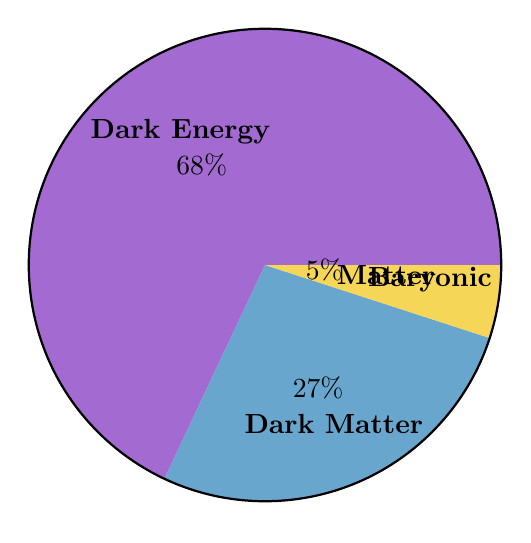
\begin{tikzpicture}
    % Pie chart
    \def\radius{3cm}
    
    % Dark Energy
    \fill[cosmicpurple!70] (0,0) -- (0:\radius) arc (0:244.8:\radius) -- cycle;
    \node at (122.4:2cm) {\textbf{Dark Energy}};
    \node at (122.4:1.5cm) {68\%};
    
    % Dark Matter
    \fill[yolyblue!70] (0,0) -- (244.8:\radius) arc (244.8:342:\radius) -- cycle;
    \node at (293.4:2.2cm) {\textbf{Dark Matter}};
    \node at (293.4:1.7cm) {27\%};
    
    % Baryonic Matter
    \fill[cosmicgold!70] (0,0) -- (342:\radius) arc (342:360:\radius) -- cycle;
    \node at (351:1.2cm) [right] {\textbf{Baryonic}};
    \node at (351:0.8cm) [right] {\textbf{Matter}};
    \node at (351:0.4cm) [right] {5\%};
    
    % Border
    \draw[thick] (0,0) circle (\radius);
\end{tikzpicture}
\end{center}

\begin{importantbox}[Cosmological Parameters (Planck 2018)]
\textbf{Energy Densities:}
\begin{itemize}
    \item Total density parameter: $\Omega_{tot} = 1.0000 \pm 0.0008$ (flat universe)
    \item Dark energy: $\Omega_\Lambda = 0.6847 \pm 0.0073$
    \item Dark matter: $\Omega_c h^2 = 0.1200 \pm 0.0012$
    \item Baryonic matter: $\Omega_b h^2 = 0.02237 \pm 0.00015$
\end{itemize}

\textbf{Expansion and Age:}
\begin{itemize}
    \item Hubble constant: $H_0 = 67.4 \pm 0.5$ km/s/Mpc
    \item Age of universe: $t_0 = 13.787 \pm 0.020$ billion years
\end{itemize}

\textbf{Primordial Fluctuations:}
\begin{itemize}
    \item Scalar spectral index: $n_s = 0.9649 \pm 0.0042$
    \item Amplitude: $A_s = 2.1 \times 10^{-9}$
    \item Optical depth (reionization): $\tau = 0.054 \pm 0.007$
\end{itemize}
\end{importantbox}

\newpage

\section{Future Observations and Open Questions}

\subsection{Next-Generation CMB Experiments}

\begin{enumerate}[leftmargin=*]
    \item \textbf{CMB-S4 (2030s)}
    \begin{itemize}
        \item Ground-based observatory with 500,000 detectors
        \item Goals: Constrain neutrino masses, test inflation models, measure gravitational lensing
    \end{itemize}
    
    \item \textbf{LiteBIRD (Launch: 2028)}
    \begin{itemize}
        \item Japanese space mission
        \item Search for B-mode polarization from primordial gravitational waves
        \item Target sensitivity: $r < 0.001$ (tensor-to-scalar ratio)
    \end{itemize}
    
    \item \textbf{Simons Observatory (Operating)}
    \begin{itemize}
        \item Ground-based in Atacama Desert, Chile
        \item High-resolution maps of CMB temperature and polarization
    \end{itemize}
\end{enumerate}

\subsection{Open Questions in Cosmology}

\begin{cosmicbox}[Major Unsolved Problems]
\begin{enumerate}
    \item \textbf{What is dark matter?}
    \begin{itemize}
        \item Direct detection experiments ongoing
        \item Particle physics beyond Standard Model required
    \end{itemize}
    
    \item \textbf{What is dark energy?}
    \begin{itemize}
        \item Cosmological constant or dynamical field?
        \item Why is its value so small compared to predictions?
    \end{itemize}
    
    \item \textbf{Did inflation occur?}
    \begin{itemize}
        \item What is the inflaton field?
        \item Detection of primordial gravitational waves would confirm
    \end{itemize}
    
    \item \textbf{What happened before the Big Bang?}
    \begin{itemize}
        \item Quantum gravity needed
        \item String theory, loop quantum gravity candidates
    \end{itemize}
    
    \item \textbf{Why is there more matter than antimatter?}
    \begin{itemize}
        \item Baryon asymmetry problem
        \item CP violation in early universe
    \end{itemize}
    
    \item \textbf{What is the fate of the universe?}
    \begin{itemize}
        \item Big Rip, Heat Death, or Big Crunch?
        \item Depends on evolution of dark energy
    \end{itemize}
\end{enumerate}
\end{cosmicbox}

\newpage

% ============= PRACTICE PROBLEMS SECTION =============

\section*{Practice Problems for Students}
\addcontentsline{toc}{section}{Practice Problems}

\begin{tcolorbox}[
    enhanced,
    colback=cosmicgold!10,
    colframe=cosmicgold,
    colbacktitle=cosmicgold,
    coltitle=black,
    fonttitle=\bfseries\Large,
    title=Instructions for Practice Problems,
    attach boxed title to top center={yshift=-3mm},
    boxed title style={sharp corners},
    sharp corners
]
These problems are designed to test your understanding of the CMB and early universe concepts. Work through them systematically, showing all calculations. Discuss your answers with your instructor.

\textbf{Difficulty levels:} $\star$ = Basic, $\star\star$ = Intermediate, $\star\star\star$ = Advanced
\end{tcolorbox}

\vspace{0.5cm}

\subsection*{Section 1: Basic Concepts and Calculations}

\begin{problem}[$\star$]
The current temperature of the CMB is measured to be $T_0 = 2.725$ K.
\begin{enumerate}[label=(\alph*)]
    \item Calculate the peak wavelength of the CMB using Wien's displacement law: $\lambda_{max} = \frac{b}{T}$ where $b = 2.898 \times 10^{-3}$ m·K.
    \item In what part of the electromagnetic spectrum does this wavelength fall?
    \item Calculate the photon number density using $n_\gamma = \frac{2\zeta(3)}{\pi^2}\left(\frac{k_BT}{\hbar c}\right)^3$ where $\zeta(3) = 1.202$.
\end{enumerate}

\textit{Working space:}
\vspace{6cm}

\textbf{Answer:}
\vspace{2cm}
\end{problem}

\begin{problem}[$\star$]
At recombination, the universe had a temperature of approximately $T_{rec} = 3000$ K and redshift $z_{rec} \approx 1090$.
\begin{enumerate}[label=(\alph*)]
    \item Using $T(z) = T_0(1 + z)$, verify that these values are consistent with today's CMB temperature.
    \item By what factor has the universe expanded since recombination?
    \item If a photon had wavelength $\lambda = 500$ nm at recombination, what is its wavelength today?
\end{enumerate}

\textit{Working space:}
\vspace{6cm}

\textbf{Answer:}
\vspace{2cm}
\end{problem}

\begin{problem}[$\star\star$]
The Hubble constant is measured as $H_0 = 67.4$ km/s/Mpc.
\begin{enumerate}[label=(\alph*)]
    \item Convert $H_0$ to SI units (s$^{-1}$). (Note: 1 Mpc = $3.086 \times 10^{22}$ m)
    \item Calculate the Hubble time: $t_H = 1/H_0$. Express your answer in years.
    \item The actual age of the universe is 13.8 billion years. Why is this different from the Hubble time?
\end{enumerate}

\textit{Working space:}
\vspace{6cm}

\textbf{Answer:}
\vspace{2cm}
\end{problem}

\newpage

\subsection*{Section 2: CMB Anisotropies and Power Spectrum}

\begin{problem}[$\star\star$]
CMB temperature fluctuations are of order $\Delta T / T \sim 10^{-5}$.
\begin{enumerate}[label=(\alph*)]
    \item If $T_0 = 2.725$ K, what is the typical magnitude of temperature fluctuations $\Delta T$ in microkelvin ($\mu$K)?
    \item The first acoustic peak in the angular power spectrum occurs at $\ell \approx 220$. Calculate the corresponding angular scale $\theta \approx 180°/\ell$.
    \item This angular scale corresponds to the sound horizon at recombination. If the sound speed in the baryon-photon plasma was $c_s \approx c/\sqrt{3}$, estimate the comoving size of the sound horizon.
\end{enumerate}

\textit{Working space:}
\vspace{8cm}

\textbf{Answer:}
\vspace{2cm}
\end{problem}

\begin{problem}[$\star\star\star$]
The acoustic oscillations in the early universe can be modeled as:
\begin{equation*}
\frac{\partial^2 \delta}{\partial t^2} + \frac{\dot{a}}{a}\frac{\partial \delta}{\partial t} = c_s^2 \nabla^2 \delta + \text{(source terms)}
\end{equation*}
where $\delta = \delta \rho / \rho$ is the density contrast.
\begin{enumerate}[label=(\alph*)]
    \item Explain physically what each term represents.
    \item In the radiation-dominated era with scale factor $a(t) \propto t^{1/2}$, show that the damping term is $\dot{a}/a = 1/(2t)$.
    \item Why do we observe multiple peaks in the CMB power spectrum?
\end{enumerate}

\textit{Working space:}
\vspace{8cm}

\textbf{Answer:}
\vspace{2cm}
\end{problem}

\newpage

\subsection*{Section 3: Cosmic Inflation}

\begin{problem}[$\star\star$]
During inflation, the scale factor grows as $a(t) = a_i e^{Ht}$ where $H$ is approximately constant.
\begin{enumerate}[label=(\alph*)]
    \item If inflation lasts for time $\Delta t = 10^{-32}$ s and $H \approx 10^{36}$ s$^{-1}$, by what factor does the universe expand during inflation?
    \item A quantum fluctuation of wavelength $\lambda_i = 10^{-35}$ m at the start of inflation is stretched by this expansion. What is its final wavelength?
    \item Compare this to the current Hubble radius $c/H_0 \approx 10^{26}$ m. Could this fluctuation be observable today?
\end{enumerate}

\textit{Working space:}
\vspace{8cm}

\textbf{Answer:}
\vspace{2cm}
\end{problem}

\begin{problem}[$\star\star\star$]
The horizon problem can be quantified by calculating the particle horizon at recombination.
\begin{enumerate}[label=(\alph*)]
    \item In a radiation-dominated universe, $a(t) \propto t^{1/2}$. The particle horizon is:
    \begin{equation*}
    d_H(t) = a(t) \int_0^t \frac{c\,dt'}{a(t')} = 2ct
    \end{equation*}
    At recombination ($t_{rec} \approx 380,000$ years), calculate $d_H(t_{rec})$.
    
    \item The proper distance to the CMB surface today is about $d_{CMB} \approx 45$ billion light-years. Calculate the angular size of the horizon at recombination as seen today: $\theta_H = d_H(t_{rec})/d_{CMB}$.
    
    \item Regions separated by more than this angle were never in causal contact. Why is the CMB uniform over larger angular scales?
\end{enumerate}

\textit{Working space:}
\vspace{10cm}

\textbf{Answer:}
\vspace{2cm}
\end{problem}

\newpage

\subsection*{Section 4: Big Bang Nucleosynthesis}

\begin{problem}[$\star$]
The neutron-to-proton ratio at the start of nucleosynthesis (T $\approx$ 0.8 MeV) is determined by thermal equilibrium:
\begin{equation*}
\frac{n}{p} = e^{-\Delta m c^2 / k_BT}
\end{equation*}
where $\Delta m = m_n - m_p = 1.293$ MeV/c$^2$.
\begin{enumerate}[label=(\alph*)]
    \item Calculate the neutron-to-proton ratio at $T = 0.8$ MeV. (Use $k_B T = 0.8$ MeV)
    \item Free neutrons decay with half-life $t_{1/2} = 10.2$ minutes. If nucleosynthesis begins at $t \approx 3$ minutes, what fraction of neutrons have decayed?
    \item Almost all remaining neutrons are incorporated into ${}^4$He. If the final $n/p$ ratio is 1/7, calculate the mass fraction of helium-4.
\end{enumerate}

\textit{Working space:}
\vspace{8cm}

\textbf{Answer:}
\vspace{2cm}
\end{problem}

\begin{problem}[$\star\star$]
The abundance of deuterium is very sensitive to the baryon density. Consider the reaction $p + n \leftrightarrow D + \gamma$.
\begin{enumerate}[label=(\alph*)]
    \item The deuterium binding energy is $B_D = 2.22$ MeV. At what temperature does deuterium formation become favorable?
    \item The "deuterium bottleneck" delays nucleosynthesis. Explain why deuterium must form before heavier elements.
    \item Observed deuterium abundance: D/H $\approx 2.5 \times 10^{-5}$. Higher baryon density leads to more deuterium burning. Is this consistent with Planck's measurement of $\Omega_b h^2 = 0.022$?
\end{enumerate}

\textit{Working space:}
\vspace{8cm}

\textbf{Answer:}
\vspace{2cm}
\end{problem}

\newpage

\subsection*{Section 5: Dark Matter and Dark Energy}

\begin{problem}[$\star\star$]
Galaxy rotation curves provide evidence for dark matter. Consider a galaxy with flat rotation curve $v(r) = v_0 = 200$ km/s for $r > 10$ kpc.
\begin{enumerate}[label=(\alph*)]
    \item Using Newton's law of gravity, $v^2 = GM(r)/r$, show that the enclosed mass grows linearly with radius: $M(r) \propto r$.
    \item Calculate the total mass enclosed within $r = 50$ kpc. (Use $G = 4.3 \times 10^{-3}$ pc (km/s)$^2$ M$_\odot^{-1}$)
    \item If visible matter accounts for only $1/6$ of this mass, what is the dark matter mass within 50 kpc?
\end{enumerate}

\textit{Working space:}
\vspace{8cm}

\textbf{Answer:}
\vspace{2cm}
\end{problem}

\begin{problem}[$\star\star\star$]
The Friedmann equation for a flat universe ($k=0$) is:
\begin{equation*}
H^2 = \frac{8\pi G}{3}(\rho_m + \rho_\Lambda)
\end{equation*}
where $\rho_m = \rho_{m,0} a^{-3}$ (matter) and $\rho_\Lambda = $ constant (dark energy).
\begin{enumerate}[label=(\alph*)]
    \item Show that $H^2 = H_0^2[\Omega_m a^{-3} + \Omega_\Lambda]$ where $\Omega_m + \Omega_\Lambda = 1$.
    
    \item The universe transitions from deceleration to acceleration when $\ddot{a} = 0$. Using the acceleration equation:
    \begin{equation*}
    \frac{\ddot{a}}{a} = -\frac{4\pi G}{3}(\rho_m + 3p_\Lambda)
    \end{equation*}
    and $p_\Lambda = -\rho_\Lambda c^2$, find the scale factor $a_{trans}$ at transition.
    
    \item For $\Omega_m = 0.3$ and $\Omega_\Lambda = 0.7$, at what redshift did acceleration begin?
\end{enumerate}

\textit{Working space:}
\vspace{10cm}

\textbf{Answer:}
\vspace{2cm}
\end{problem}

\newpage

\subsection*{Section 6: Advanced Integration Problems}

\begin{problem}[$\star\star\star$]
The energy density of the CMB is given by the Stefan-Boltzmann law:
\begin{equation*}
\rho_{CMB} = \frac{4\sigma T^4}{c^3} = \frac{\pi^2 k_B^4}{15\hbar^3 c^3}T^4
\end{equation*}
\begin{enumerate}[label=(\alph*)]
    \item Calculate the current energy density of the CMB for $T_0 = 2.725$ K. Express in J/m$^3$ and eV/cm$^3$.
    
    \item At what redshift was the energy density of CMB photons equal to the critical density today ($\rho_c = 9.5 \times 10^{-27}$ kg/m$^3$)?
    
    \item Matter density scales as $\rho_m \propto a^{-3}$ while radiation scales as $\rho_r \propto a^{-4}$. At what redshift were matter and radiation densities equal (matter-radiation equality)?
\end{enumerate}

\textit{Working space:}
\vspace{10cm}

\textbf{Answer:}
\vspace{2cm}
\end{problem}

\begin{problem}[$\star\star\star$]
The comoving distance to an object at redshift $z$ is:
\begin{equation*}
\chi(z) = \frac{c}{H_0}\int_0^z \frac{dz'}{E(z')}
\end{equation*}
where $E(z) = \sqrt{\Omega_m(1+z)^3 + \Omega_\Lambda}$.
\begin{enumerate}[label=(\alph*)]
    \item For a flat universe with $\Omega_m = 0.3$ and $\Omega_\Lambda = 0.7$, set up (but don't solve) the integral for the comoving distance to the CMB surface at $z = 1090$.
    
    \item The angular diameter distance is $d_A = \chi/(1+z)$. Calculate $d_A$ for the CMB. (You may use numerical integration or approximation)
    
    \item The sound horizon at recombination subtends angle $\theta = 0.6°$. What is the physical size of the sound horizon in Mpc?
\end{enumerate}

\textit{Working space:}
\vspace{10cm}

\textbf{Answer:}
\vspace{2cm}
\end{problem}

\newpage

\subsection*{Section 7: Conceptual Questions}

\begin{problem}[$\star\star$]
Answer the following conceptual questions with clear explanations:
\begin{enumerate}[label=(\alph*)]
    \item Why is the CMB a blackbody spectrum? What process established thermal equilibrium in the early universe?
    
    \item Explain why the CMB is redshifted, but still maintains a blackbody spectrum (hint: discuss adiabatic expansion).
    
    \item The CMB is nearly isotropic, but there's a dipole anisotropy of order $\Delta T/T \sim 10^{-3}$. What causes this dipole?
\end{enumerate}

\textit{Working space:}
\vspace{10cm}

\textbf{Answer:}
\vspace{2cm}
\end{problem}

\begin{problem}[$\star\star\star$]
Consider the following statements and explain whether each is true or false:
\begin{enumerate}[label=(\alph*)]
    \item "The CMB represents the surface of last scattering, so we are looking at a 2D shell around us." 
    
    \item "If inflation never occurred, we would still observe the CMB, but it would have different properties."
    
    \item "Dark energy and dark matter are both 'dark' because they don't emit light, so they might be related."
    
    \item "The temperature fluctuations in the CMB are caused by quantum fluctuations that occurred during inflation."
\end{enumerate}

\textit{Working space:}
\vspace{12cm}

\textbf{Answer:}
\vspace{2cm}
\end{problem}

\newpage

\subsection*{Section 8: Research-Based Questions}

\begin{problem}[$\star\star\star$]
\textbf{Project Question:} Research and write a short report (2-3 pages) on one of the following topics:
\begin{enumerate}[label=(\alph*)]
    \item The Planck satellite mission: instruments, observations, and key discoveries
    \item The search for primordial gravitational waves (B-mode polarization)
    \item The Hubble tension: different measurements of $H_0$ and implications
    \item The lithium problem in Big Bang nucleosynthesis
\end{enumerate}

Your report should include:
\begin{itemize}
    \item Historical background
    \item Current observational status
    \item Theoretical implications
    \item Future prospects
    \item At least 5 references
\end{itemize}

\textit{Working space:}
\vspace{2cm}
\end{problem}

\vspace{1cm}

\begin{tcolorbox}[
    enhanced,
    colback=yolylightblue,
    colframe=yolyblue,
    colbacktitle=yolyblue,
    coltitle=white,
    fonttitle=\bfseries,
    title=Additional Resources,
    sharp corners
]
\textbf{Recommended Textbooks:}
\begin{itemize}
    \item Ryden, B. "Introduction to Cosmology" (2nd Edition)
    \item Dodelson, S. \& Schmidt, F. "Modern Cosmology" (2nd Edition)
    \item Weinberg, S. "Cosmology"
\end{itemize}

\textbf{Online Resources:}
\begin{itemize}
    \item Planck Mission Results: \url{http://www.cosmos.esa.int/web/planck}
    \item Particle Data Group: \url{http://pdg.lbl.gov}
    \item NASA's WMAP Tutorial: \url{http://map.gsfc.nasa.gov}
\end{itemize}

\textbf{Video Lectures:}
\begin{itemize}
    \item Leonard Susskind's Cosmology Lectures (Stanford)
    \item Sean Carroll's "The Big Picture" Lectures
\end{itemize}
\end{tcolorbox}

\newpage

% ============= CLOSING PAGE =============

\thispagestyle{empty}

\vspace*{\fill}

\begin{center}
\begin{tcolorbox}[
    width=0.9\textwidth,
    enhanced,
    colback=yolyblue,
    colframe=cosmicgold,
    boxrule=3pt,
    arc=5mm
]
\centering
{\Huge\textcolor{white}{\textbf{Yolymatics Tutorials}}}\\[0.5cm]
{\Large\textcolor{white}{\textit{Inspiring Excellence in Physics \& Mathematics}}}
\end{tcolorbox}

\vspace{1cm}

\begin{tcolorbox}[
    width=0.9\textwidth,
    colback=white,
    colframe=yolyblue,
    boxrule=2pt,
    sharp corners
]
\centering
\textbf{Contact Information}\\[0.3cm]
\textcolor{yolyblue}{\Large\href{http://www.yolymaticstutorials.com}{www.yolymaticstutorials.com}}\\[0.5cm]

\begin{tabular}{rl}
\textbf{Email:} & admin@yolymaticstutorials.com \\
\textbf{Phone:} & +27 84 759 7313 \\
\textbf{Location:} & South Africa \\
\end{tabular}
\end{tcolorbox}

\vspace{1cm}

\begin{tcolorbox}[
    width=0.9\textwidth,
    colback=yolylightblue!30,
    colframe=yolyblue,
    sharp corners
]
\centering
\textbf{Our Services:}\\[0.3cm]
\begin{tabular}{c c c}
A-Level Tutoring & University Preparation & Research Mentoring \\
Online Classes & Study Materials & Exam Preparation \\
\end{tabular}
\end{tcolorbox}

\vspace{1cm}

{\large\textit{"Understanding the universe begins with curiosity"}}

\end{center}

\vspace*{\fill}

\begin{center}

\begin{tikzpicture}
    \fill[yolydarkblue] (0,0) rectangle (15,0.1);
    \fill[cosmicgold] (0,0.1) rectangle (15,0.2);
\end{tikzpicture}
\end{center}

\end{document}
